\documentclass[a4paper,ngerman,12pt]{scrartcl}

\usepackage[utf8]{inputenc}

\usepackage[ngerman]{babel}

\usepackage{amsmath,amsthm,amssymb,stmaryrd,color,graphicx,mathtools}
\usepackage{array}
\usepackage[all]{xy}

\usepackage{shadethm}

\usepackage[protrusion=true,expansion=true]{microtype}

\usepackage[T1]{fontenc}
\usepackage{libertine}

\usepackage{hyperref}

\setlength{\shadeboxsep}{6pt}
\setlength{\shadeleftshift}{-\shadeboxsep}
\setlength{\shaderightshift}{-\shadeboxsep}

\theoremstyle{definition}
\newtheorem{defn}{Definition}[section]
%\newtheorem{defn}{Definition}[section]
\newtheorem{ex}[defn]{Beispiel}
\newtheorem{motto}[defn]{Motto}

\theoremstyle{plain}

\newtheorem{defnprop}[defn]{Definition/Proposition}
\newtheorem{prop}[defn]{Proposition}
\newtheorem{fact}[defn]{Fakt}
\newtheorem{lemma}[defn]{Lemma}
\newtheorem{thm}[defn]{Satz}
\newtheorem{cor}[defn]{Korollar}

\theoremstyle{remark}
\newtheorem{rem}[defn]{Bemerkung}
\newtheorem{warning}[defn]{Warnung}

\clubpenalty=10000
\widowpenalty=10000
\displaywidowpenalty=10000

\renewcommand{\AA}{\mathbb{A}}
\newcommand{\CC}{\mathbb{C}}
\newcommand{\NN}{\mathbb{N}}
\newcommand{\ZZ}{\mathbb{Z}}
\newcommand{\QQ}{\mathbb{Q}}
\newcommand{\FF}{\mathbb{F}}
\newcommand{\PP}{\mathbb{P}}
\newcommand{\C}{\mathcal{C}}
\newcommand{\E}{\mathcal{E}}
\newcommand{\F}{\mathcal{F}}
\newcommand{\G}{\mathcal{G}}
\renewcommand{\H}{\mathcal{H}}
\newcommand{\N}{\mathcal{N}}
\newcommand{\J}{\mathcal{J}}
\newcommand{\K}{\mathcal{K}}
\renewcommand{\L}{\mathcal{L}}
\renewcommand{\O}{\mathcal{O}}
\newcommand{\id}{\mathrm{id}}
\newcommand{\op}{\mathrm{op}}
\newcommand{\ppp}{\mathfrak{p}}
\newcommand{\mmm}{\mathfrak{m}}
\newcommand{\xra}[1]{\xrightarrow{#1}}
\newcommand{\Mod}{\mathrm{Mod}}
\newcommand{\Set}{\mathrm{Set}}
\newcommand{\Cat}{\mathrm{Cat}}
\newcommand{\Vect}{\mathrm{Vect}}
\newcommand{\VB}{\mathrm{VB}}
\newcommand{\Id}{\mathrm{Id}}
\newcommand{\Coh}{\mathrm{Coh}}
\newcommand{\GL}{\mathrm{GL}}
\newcommand{\pt}{\mathrm{pt}}
\newcommand{\Ob}{\operatorname{Ob}}
\newcommand{\rank}{\operatorname{rank}}
\newcommand{\Hom}{\mathrm{Hom}}
\newcommand{\Pic}{\mathrm{Pic}}
\newcommand{\ul}[1]{\underline{#1}}
\newcommand{\placeholder}{\underline{\ \ }}
\newcommand{\lra}{\longrightarrow}
\renewcommand{\div}{\operatorname{div}}
\newcommand{\Div}{\mathrm{Div}}
\newcommand{\ord}{\operatorname{ord}}
\newcommand{\PD}{\operatorname{PD}}
\newcommand{\Sh}{\operatorname{Sh}}
\DeclareMathOperator{\Spec}{Spec}
\DeclareMathOperator{\Proj}{Proj}
\DeclareMathOperator{\Sym}{Sym}
\DeclareMathOperator{\colim}{colim}
\newcommand{\defeq}{\vcentcolon=}
\newcommand{\defeqv}{\vcentcolon\equiv}

\begin{document}

\title{Quasikohärente Modulgarben}
\author{Ingo Blechschmidt}
\date{28. Mai 2015}
\maketitle

\section{Definitionen}

\begin{defn}Eine~($\O_X$-)Modulgarbe auf einem geringten Raum~$(X,\O_X)$ besteht
aus \ldots{} sodass \ldots\end{defn}

\begin{defn}Eine Modulgarbe~$\E$ heißt genau dann \emph{lokal endlich frei},
wenn \ldots{} Sie heißt genau dann \emph{von endlichem Typ}, wenn
\ldots\end{defn}

\begin{rem}Die Kategorie~$\mathrm{Mod}(\O_X)$ der~$\O_X$-Modulgarben ist
abelsch, vollständig und kovollständig und sogar eine
Grothendieck-Kategorie.\end{rem}

\begin{rem}Aus Sicht der internen Sprache des Topos~$\Sh(X)$ ist
eine~$\O_X$-Modulgarbe nichts anderes als ein gewöhnlicher Modul über dem
gewöhnlichen Ring~$\O_X$. Sie ist genau dann lokal endlich frei, wenn sie aus
interner Sicht endlich frei ist. Sie ist genau dann von endlichem Typ, wenn sie
aus interner Sicht endlich erzeugt ist.\end{rem}


\section{Beispiele}

\begin{defnprop}Sei~$M$ ein~$A$-Modul. Dann gibt es auf~$\Spec A$ eine
Modulgarbe~$M^\sim$ mit
\begin{enumerate}
\item $M^\sim(D(f)) \cong M[f^{-1}]$ für alle~$f \in A$ und
\item $(M^\sim)_\ppp \cong M_\ppp = M[(A\setminus\ppp)^{-1}]$ für alle~$\ppp
\in \Spec A$.
\end{enumerate}
\end{defnprop}

\begin{rem}Im Topos~$\Sh(\Spec A)$ gibt es den \emph{generischen Filter}~$\F$,
die Untergarbe der konstanten Garbe~$\ul{A}$ mit~$\F(U) \defeq \{ f : U \to A
\,|\, \text{$f(\ppp) \not\in \ppp$ für alle~$\ppp \in U$} \}$. Aus interner
Sicht ist dann~$M^\sim$ einfach die Lokalisierung~$\ul{M}[\F^{-1}]$.\end{rem}

\begin{ex}$A^\sim \cong \O_{\Spec A}$.\end{ex}

\begin{ex}Die Garbe~$(k[x,y]/(x-2,y-3))^\sim$ auf~$\Spec k[x,y]$ ist im
Punkt~$(x-2,y-3)$ konzentriert, d.\,h. die Menge derjenigen Punkte, an denen
der Halm dieser Garbe nicht Null ist, enthält nur diesen einen Punkt. Daher
heißt eine solche Garbe auch \emph{Wolkenkratzergarbe}.\end{ex}

\begin{prop}Sei~$M$ ein~$A$-Modul. Genau dann ist~$M^\sim$ lokal endlich frei,
wenn~$M$ endlich erzeugt und projektiv ist.\end{prop}

\begin{ex}Seien~$M$ und~$N$ quadratische~$(n \times n)$-Matrizen über einem
Körper~$k$. Eine notwendige Bedingung dafür, dass~$M$ und~$N$ zueinander
ähnlich sind, ist, dass ihr Spektrum übereinstimmt. Bekanntlich ist diese
Bedingung aber nicht hinreichend.

Eine Charakterisierung von Ähnlichkeit ist
mit~$k[X]$-Moduln möglich: Genau dann sind~$M$ und~$N$ zueinander ähnlich, wenn
die~$k[X]$-Moduln~$k^n_M$ und~$k^n_N$ zueinander isomorph sind. (Als
abelsche Gruppe ist~$k^n_M = k^n$. Die Skalarmultiplikation ist definiert
als~$f \cdot v \defeq f(M)v$.) Das ist genau dann der Fall, wenn die
induzierten Modulgarben~$(k^n_M)^\sim$ und~$(k^n_N)^\sim$ auf~$\AA^1_k = \Spec
k[X]$ isomorph sind. Man kann sich nun überlegen, dass diese Garben Träger im
Spektrum haben.

Fazit: Wir können die Modulgarbe~$(k^n_M)^\sim$ als Verfeinerung der noch zu
groben Invariante des Spektrums deuten. Sie kodiert genau den Ähnlichkeitstyp
von~$M$.\end{ex}

\begin{defn}Die \emph{Faser} einer Modulgarbe~$\E$ über einem Punkt~$x$ ist
der~$k(x)$-Vektorraum
\[ \E|_x \defeq \E_x \otimes_{\O_{X,x}} k(x) \cong \E_x/\mmm_x \E_x. \]
\end{defn}

Ist~$s \in \E(U)$ ein lokaler Schnitt einer Modulgarbe, so ist für jeden
Punkt~$x \in U$ die Restklasse von~$s$ in~$\E|_x$ ein Element eines (von~$x$
abhängigen) Vektorraums. In diesem Sinn kann man Schnitte von Modulgarben als
\emph{verallgemeinerte Funktionen} betrachten. Diese sind wichtig, da es
interessanten Schemata oftmals an globalen gewöhnlichen Funktionen -- globalen
Schnitten von~$\O_X$ -- mangelt.

\begin{ex}Sei~$W$ ein endlich-dimensionaler~$k$-Vektorraum und~$X = \PP(W) =
\Proj \Sym W^\vee$ seine Projektivierung. Die~$k$-rationalen Punkte dieses
Schemas sind gerade die eindimensionalen Unterräume von~$W$. Auf~$X$ gibt es
die wichtigen Modulgarben~$\O(1)$ und~$\O(-1)$. Für die Fasern dieser Garben an
einem Punkt~$\ell \subseteq W$ gilt
\[ \O(1)|_\ell \cong \ell^\vee \qquad\text{und}\qquad \O(-1)|_\ell \cong \ell. \]
Die Garbe~$\O(-1)$ heißt daher auch \emph{tautologisches Bündel}.

In Skizzen kann man die beiden Garben nicht unterscheiden -- wenn man~$X$ als
Kreis zeichnet ($\dim W = 2$), so sehen beide wie das Möbiusbündel aus. Als
Garben sind sie aber nicht isomorph; das tautologische Bündel hat nur den
Nullschnitt als globalen Schnitt, während~$\O(1)(X)$ kanonisch isomorph
zu~$W^\vee$ ist.

Allgemeiner gibt es für alle~$m \in \ZZ$ jeweils eine besondere
Modulgarbe~$\O(m)$; für die globalen Schnitte gilt~$\O(m)(X) \cong \Sym^m
W^\vee$.\end{ex}

\begin{ex}Sei~$D$ ein Cartier-Divisor auf einem Schema~$X$. Dann ist die
Untermodulgarbe
\[ \O_X(D) \defeq \{ f : \K_X \,|\, \mathrm{div}(f) + D \geq 0 \} \]
der Garbe der rationalen Funktionen lokal frei vom Rang~1. Die Signifikanz
dieser Garben erklärt sich dadurch, dass in vielen Situationen jede Modulgarbe,
die lokal frei vom Rang~1 ist, von dieser Form ist; und dass man sie verwenden
kann, um Schnitttheorie zu betreiben: Ist~$X$ eine Fläche, so ist die
Schnittzahl zweier Divisoren~$D$ und~$D'$ gleich
\[ (D \cdot D') \defeq \chi(\O_X) - \chi(\O_X(-D)) - \chi(\O_X(-D')) + \chi(\O_X(-D-D')). \]
Dabei berechnet~$\chi$ die \emph{Euler-Charakteristik} einer (kohärenten)
Garbe.
\end{ex}

\begin{ex}Sei~$\E$ eine lokal freie Modulgarbe vom Rang~$n$. Solche Garben
heißen auch \emph{Vektorbündel}. In der Tat kann man aus einer solchen Garbe
ein Vektorbündel im eigentlichen Sinn konstruieren, nämlich den
Morphismus~$\ul{\Spec}_X \Sym \E^\vee \to X$.\end{ex}

\begin{ex}Wie kann man einen Morphismus~$X \to \PP^n$ angeben? Naiv erwartet
man, dass eine Setzung der Form~$x \mapsto [s_0(x) : \cdots : s_n(x)]$ Erfolg
haben sollte, solange die~$s_i$ nirgends gemeinsam verschwinden. Aber was
können die~$s_i$ sein? Sich hier auf globale Funktionen zu beschränken wäre
sehr restriktiv -- auf vielen interessanten Schemata gibt es nur wenige globale
Funktionen. Tatsächlich genügt es, wenn die~$s_i$ globale Schnitte eines
Geradenbündels auf~$X$ sind, also einer lokal freien Modulgarbe vom Rang~1.\end{ex}

\begin{rem}Das vorherige Beispiel kann man zu einer universellen Eigenschaft
des projektiven Raums verbessern: Für lokal geringte Räume~$X$ stehen die
Morphismen~$X \to \PP^n$ in kanonischer Eins-zu-Eins-Korrespondenz mit
Geradenbündeln~$\L$ auf~$X$ zusammen mit~$n + 1$ globalen Schnitten, welche
nirgends gemeinsam verschwinden, bis auf Isomorphie. Kurz:
\[ \Hom(X, \PP^n) \cong \{ (\L,\,\O_X^{n+1} \twoheadrightarrow \L) \}/{\cong}. \]
\end{rem}

\begin{ex}Sei~$X$ ein Schema über~$S$. Dann gibt es auf~$X$ die
Modulgarbe~$\Omega^1_{X/S}$ der relativen Kählerdifferentialformen.\end{ex}

\begin{ex}Sei~$V(\J) \hookrightarrow X$ ein abgeschlossenes Unterschema. Dann
hat die Garbe~$\J/\J^2$ nur Träger in~$V(\J)$, kann also auch als Garbe
auf~$V(\J)$ angesehen werden. Als solche heißt sie \emph{Konormalgarbe}
von~$V(\J)$ in~$X$. Wenn~$\J$ lokal von regulären Sequenzen der Länge~$r$
erzeugt wird, ist sie lokal frei vom Rang~$r$.\end{ex}


\section{Operationen mit Modulgarben}

\begin{defn}Seien~$\E$ und~$\F$ Modulgarben auf einem geringten Raum~$(X,\O_X)$. Dann
sind~$\E \oplus \F$ und~$\E \otimes_{\O_X} \F$ definiert als \ldots\end{defn}

\begin{rem}Aus der internen Sicht des Topos~$\Sh(X)$ sind direkte Summe und
Tensorprodukt von Modulgarben einfach durch die gewöhnliche direkte Summe und
das gewöhnliche Tensorprodukt von gewöhnlichen Moduln gegeben.\end{rem}

\begin{defn}Sei~$f : X \to Y$ ein Morphismus von geringten Räumen. Ist~$\E$
eine Modulgarbe auf~$Y$, so ist ihr \emph{Rückzug} die Modulgarbe~$f^*\E \defeq
f^{-1}\E \otimes_{f^{-1}\O_Y} \O_X$ auf~$X$. Ist~$\F$ eine Modulgarbe auf~$X$,
so ist ihr \emph{Pushforward} die Modulgarbe~$f_*\F$ auf~$Y$.\end{defn}

\begin{rem}$f^* \dashv f_*$.\end{rem}

\begin{rem}Für die Halme des Rückzugs gibt es die einfache Formel~$(f^*\E)_x
\cong \E_{f(x)} \otimes_{\O_{Y,f(x)}} \O_{X,x}$. Für die Halme des Pushforwards
gibt es die Formel~$(f_*\F)_y \cong \colim_{f^{-1}[y] \subseteq U} \F(U)$,
welche für (im topologischen Sinn) abgeschlossene stetige Abbildungen~$f$
gültig ist.\end{rem}


\section{Quasikohärente Modulgarben}

\begin{motto}Nur die quasikohärenten Modulgarben auf einem Schema haben
geometrische Bedeutung. Die anderen sind Artefakt der Kodierung über lokal
geringte Räume.\end{motto}

\begin{defn}Sei~$X$ ein Schema und~$\E$ eine~$\O_X$-Modulgarbe. Genau dann
heißt~$\E$ \emph{quasikohärent}, wenn es lokal exakte Sequenzen der Form
\[ \O_X^{\oplus I} \lra \O_X^{\oplus J} \lra \E \lra 0 \]
gibt. Dabei können~$I$ und~$J$ beliebige, auch unendlich große, Mengen sein.
\end{defn}

\begin{prop}Sei~$X$ ein Schema und~$\E$ eine~$\O_X$-Modulgarbe. Dann sind
äquivalent:
\begin{enumerate}
\item Die Modulgarbe $\E$ ist quasikohärent.
\item Es gibt eine Überdeckung von~$X$ durch offene affine Teilmengen~$U$ sodass
für jede Überdeckungsmenge~$U = \Spec A$ die Einschränkung~$\E|_U$ isomorph zu
einer Modulgarbe der Form~$M^\sim$ für einen~$A$-Modul~$M$ ist.
\item Für alle offenen affinen Teilmengen~$U = \Spec A$ ist~$\E|_U$ isomorph zu einer
Modulgarbe der Form~$M^\sim$ für einen~$A$-Modul~$M$.
\item Für alle offenen affinen Teilmengen~$U = \Spec A$ und Funktionen~$f \in
A$ ist die kanonische Abbildung~$\E(U)[f^{-1}] \to \E(D(f))$ ein Isomorphismus
von~$A[f^{-1}]$-Moduln.
\end{enumerate}
\end{prop}

\begin{rem}Eine Modulgarbe~$\E$ auf einem Schema~$X$ ist genau dann
quasikohärent, wenn aus Sicht der internen Sprache des Topos~$\Sh(X)$ für
alle~$f : \O_X$ der lokalisierte Modul~$\E[f^{-1}]$ eine Garbe bezüglich der
Modalität~$\Box$ mit~$\Box\varphi \defeqv (\text{$f$ inv.} \Rightarrow
\varphi)$ ist.\end{rem}

\begin{ex}Die Kategorie der quasikohärenten Modulgarben auf einem affinen
Schema~$\Spec A$ ist äquivalent zur Kategorie der~$A$-Moduln. Die Äquivalenz
wird vermittelt durch den Funktor~$\E \mapsto \E(\Spec A)$ mit
Pseudoinversem~$M \mapsto M^\sim$.\end{ex}

\begin{ex}Die Kategorie der quasikohärenten Modulgarben auf einem projektiven
Schema~$\Proj A$ ist äquivalent zum Quotient der Kategorie der
$\ZZ$-graduierten~$A$-Moduln modulo der Serreschen Unterkategorie derjenigen
graduierten Moduln, welche ab einem gewissen Grad verschwinden. Die Äquivalenz
wird durch eine projektive Variante der Tilde-Konstruktion vermittelt.\end{ex}

\begin{ex}Der Rückzug quasikohärenter Modulgarben ist stets wieder
quasikohärent. Der Pushforward einer quasikohärenten Modulgarbe längs einem
quasikompakten und quasiseparierten Morphismus ist wieder
quasikohärent.\end{ex}

\begin{prop}Sei~$f : \Spec A \to \Spec B$ ein Morphismus affiner Schemata.
Betrachte~$A$ vermöge~$f^\sharp$ als~$B$-Algebra.
\begin{enumerate}
\item Sei~$M$ ein~$A$-Modul. Dann gilt~$f_*(M^\sim) \cong (M_B)^\sim$.
\item Sei~$N$ ein~$B$-Modul. Dann gilt~$f^*(N^\sim) \cong (N \otimes_B
A)^\sim$.
\end{enumerate}
\end{prop}

\begin{rem}Aus der Kategorie der quasikohärenten Modulgarben auf einem
Schema~$X$ zusammen mit ihrer abelschen Struktur kann man das Schema
rekonstruieren; das besagt der Rekonstruktionssatz von Gabriel--Rosenberg. Für
affine Schemata folgt das aus der für Ringe~$A$ gültigen Isomorphiekette
\[ A \cong \mathrm{End}(\mathrm{Id}_{\mathrm{Mod}(A)})
  \cong \mathrm{End}(\mathrm{Id}_{\mathrm{QCoh}(\Spec A)}). \]
Allgemein heißt für eine abelsche Kategorie~$\C$ die Menge der Endomorphismen
des Identitätsfunktors auf~$\C$ auch \emph{Zentrum von~$\C$}. Mit der Addition
und Verkettung von natürlichen Transformationen wird diese zu einem
kommutativen Ring.
\end{rem}

\begin{rem}Die Kategorie~$\mathrm{QCoh}(X)$ der quasikohärenten Modulgarben ist
eine koreflektive Unterkategorie der Kategorie~$\mathrm{Mod}(\O_X)$
aller Modulgarben, das heißt die Inklusion~$\mathrm{QCoh}(X) \hookrightarrow
\mathrm{Mod}(\O_X)$ besitzt einen Rechtsadjungierten, den so genannten
\emph{Kohärator}. Als Konsequenz kann man zeigen, dass~$\mathrm{QCoh}(X)$ wie
auch~$\mathrm{Mod}(\O_X)$ eine Grothendieck-Kategorie ist. Kolimiten berechnet
man in~$\mathrm{QCoh}(X)$ genau wie in~$\mathrm{Mod}(\O_X)$. Limiten
in~$\mathrm{QCoh}(X)$ berechnet man, indem man sie zunächst
in~$\mathrm{Mod}(\O_X)$ bestimmt und dann den Kohärator anwendet. Für
endliche Limiten kann man auf den Kohärator verzichten.\footnote{Seien~$M_i$
Moduln über~$A$. Das Produkt der~$M_i^\sim$ in der Kategorie aller Modulgarben
auf~$\Spec A$ ist dann eine Garbe mit~$D(f) \mapsto \prod_i M_i[f^{-1}]$.
Dagegen ist das Produkt der~$M_i^\sim$ in der Kategorie der quasikohärenten
Modulgarben eine Garbe mit~$D(f) \mapsto (\prod_i M_i)[f^{-1}]$. Es gibt zwar
einen kanonischen Morphismus~$(\prod_i M_i)[f^{-1}] \to \prod_i M_i[f^{-1}]$;
im Allgemeinen ist dieser jedoch weder injektiv noch surjektiv.}\end{rem}

%\begin{rem}Im Allgemeinen sind Kategorien von quasikohärenten Modulgarben nicht
%äquivalent zu Kategorien von Moduln über gewöhnlichen Ringen. Zum Beispiel ist
%die Kategorie der (nicht nur quasikohärenten, sondern sogar) kohärenten
%Modulgarben auf einer vollständigen Varietät über einem algebraisch
%abgeschlossenen Körper stets eine Krull--Schmidt-Kategorie.
%\end{rem}


\section{Tiefere kategorielle Interpretation}

Sei~$\E$ eine quasikohärente Modulgarbe auf einem Schema~$X$. Dann erhalten wir
für jeden Morphismus~$f : \Spec A \to X$ durch Betrachtung des Rückzugs~$f^*\E$
einen~$A$-Modul, den wir~"`$\ul{\E}(A)$"' bezeichnen möchten. In der Notation
unterdrücken wir also den Morphismus~$f$ und notieren nur seine Quelle.
Ist~$p : \Spec B \to \Spec A$ ein weiterer Morphismus, so gibt es eine
kanonische Abbildung~$\ul{\E}(A) \to \ul{\E}(B)$. Insgesamt definiert daher die
Zuordnung~$(\Spec A \to X) \mapsto \ul{\E}(A)$ eine \emph{Prägarbe} auf der
Kategorie~$\mathrm{Aff}/X$ der affinen Schemata über~$X$.

Die Familie dieser Moduln~$\ul{\E}(A)$ hat drei Besonderheiten:
\begin{enumerate}
\addtocounter{enumi}{-1}
\item Die Prägarbe~$\ul{\E}$ ist ein Modulobjekt über dem
Ringobjekt~$\ul{\O_X}$, das ist die Prägarbe
\[ \begin{array}{@{}rcl@{}}
  (\mathrm{Aff}/X)^\op &\lra& \Set \\
  (\Spec A \to X) &\longmapsto& A.
\end{array} \]
\item Seien Morphismen~$f : \Spec A \to X$ und~$p : \Spec B \to \Spec A$ gegeben. Dann
gibt es einen kanonischen Isomorphismus
\[ \ul{\E}(A) \otimes_A B \stackrel{\cong}{\lra} \ul{\E}(B), \]
denn~$p^* f^* \E$ ist kanonisch isomorph zu~$(f \circ p)^*\E$.
Diese Isomorphismen erfüllen ihrerseits eine Kohärenzbedingung.

\item Sei~$f : \Spec A \to X$ ein Morphismus und sei~$\Spec A$ überdeckt durch
offene affine Unterschemata~$\Spec A[f_i^{-1}]$. Dann ist das Diagramm
\[ \ul{\E}(A) \to \prod_i \ul{\E}(A[f_i^{-1}]) \rightrightarrows \prod_{i,j}
\ul{\E}(A[f_i^{-1},f_j^{-1}]) \]
ein Differenzkerndiagramm. Man sagt auch, die Zuordnung~$(\Spec A \to X)
\mapsto \ul{\E}(A)$ sei eine \emph{Zariski-Garbe}.
\end{enumerate}

Man kann sich überlegen, dass für eine Prägarbe~$\F$ auf~$\mathrm{Aff}/X$
Eigenschaft~2 schon aus den Eigenschaften~0 und~1 folgt. Denn das fragliche Diagramm ist
dann isomorph zu
\[ \F(A) \to \prod_i \F(A)[f_i^{-1}] \rightrightarrows \prod_{i,j}
\F(A)[f_i^{-1},f_j^{-1}], \]
und es ist eine elementare Beobachtung aus der linearen Algebra über Ringen,
dass dieses ein Differenzkerndiagramm ist.

Als Zwischenfazit halten wir fest: Eine quasikohärente Modulgarbe~$\E$
definiert ein kohärentes System von Moduln~$(\ul{\E}(A))_{\Spec A \to X}$, also ein
System, das Eigenschaft~1 hat. Umgekehrt kann man sich überlegen, dass jedes
solche System auch eine quasikohärente Modulgarbe festlegt.

Die Kategorie der quasikohärenten Modulgarben auf~$X$ ist also äquivalent zur
Kategorie der kohärenten~$\mathrm{Aff}/X$-indizierten Systeme von Moduln. Das kann
einen an die Konstruktion von Limiten in der Kategorie der Mengen erinnern!
Tatsächlich gilt
\[ \mathrm{QCoh}(X) = \lim\nolimits_{\Spec A \to X} \mathrm{Mod}(A). \]
Der Limes auf der rechten Seite muss in einem 2-kategoriellen Sinn verstanden
werden; ein Objekt dieser Kategorie besteht aus
\begin{enumerate}
\item einer Familie von Moduln: für jeden Morphismus~$\Spec A \to X$
einen~$A$-Modul~$M_A$, und
\item Isomorphismen: für jeden Morphismus~$\Spec A \to X$ und jeden
Morphismus~$\Spec B \to \Spec A$ einen Isomorphismus~$M_A \otimes_A B \to
M_B$,
\end{enumerate}
sodass diese bezüglich weiterer Morphismen~$\Spec C \to \Spec B$ ein
Kohärenzaxiom erfüllen.

Die rechte Seite kann man als Instanz der \emph{Limesformel für
Rechts-Kan-Erweiterungen} erkennen. Damit können wir also auch schreiben:
\[ \mathrm{QCoh} = \mathrm{Ran}_\mathrm{inkl}(\mathrm{Mod}). \]
Der Funktor~$\mathrm{QCoh}$, der einem Schema seine Kategorie quasikohärenter
Modulgarben zuordnet, ist also die Rechts-Kan-Erweiterung des
Funktors~$\mathrm{Mod} : \mathrm{Ring} \to \mathrm{Cat}$ (welcher einem
Ring~$A$ die Kategorie der~$A$-Moduln zuordnet) längs der
Inklusion~$\mathrm{inkl} : \mathrm{Aff}^\op \to \mathrm{Sch}^\op$;
bedenke~$\mathrm{Aff}^\op = \mathrm{Ring}$.

Man kann diese Geschichte auch noch anders erzählen. Angenommen, wir fangen
gerade an, die Grundzüge der Schematheorie zu entwickeln. Als einleuchtendes
Konzept für quasikohärente Modulgarben auf affinen Schemata~$\Spec A$ fällt uns
dann die Kategorie der gewöhnlichen~$A$-Moduln ein. Auf diese Weise erhalten
wir einen Funktor~$\mathrm{Mod} : \mathrm{Aff}^\op \to \mathrm{Cat}$. Wenn es
nun doch nur eine Möglichkeit gäbe, diesen Funktor längs der
Inklusion~$\mathrm{Aff}^\op \to \mathrm{Sch}^\op$ zu erweitern!

\begin{center}
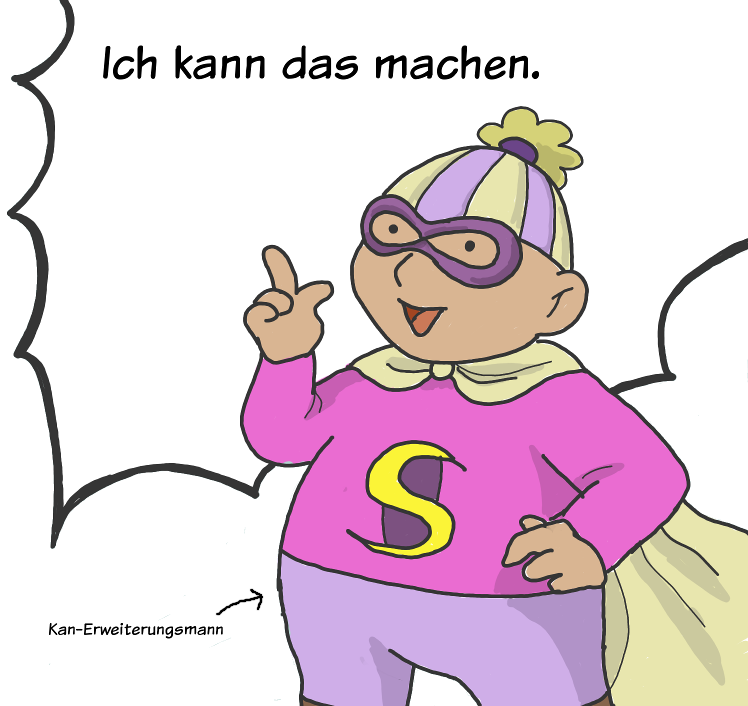
\includegraphics[scale=0.28]{kan-erweiterungsmann}
\end{center}

Beide der Ausdrücke für~$\mathrm{QCoh}(X)$ lassen sich auf Objekte~$X$
verallgemeinern, die nicht Schemata im engeren Sinn sind: zum Beispiel Garben
auf~$\mathrm{Ring}^\op$, welche nicht unbedingt lokal affin sind, oder sogar
Prägarben auf~$\mathrm{Ring}^\op$. Die Limesformel ist auch eine zentrale Idee
zur Definition der Kategorie der quasikohärenten Modulgarben auf einem Stack.

Wer mag, kann die Formel auch noch zu
\[ \mathrm{QCoh}(X) = \int_A \mathrm{Mod}(A)^{\Hom(\Spec A, X)} =
  \int_A [\ul{X}(A), \mathrm{Mod}(A)] \]
umschreiben. Damit endet unser Ausflug in die 2-kategorielle Interpretation
quasikohärenter Modulgarben.

\end{document}

* Mengentheoretische Überlegungen
* QCoh(X) = lim_i QCoh(U_i) bei offenen Überdeckungen
* ???
* ???

Limes-Formel steht auch in:
http://www.math.harvard.edu/~gaitsgde/GL/QCohBook.pdf
